% 2011_zhejiang_liberal_q7_optA: cuboid + triangular wedge on top
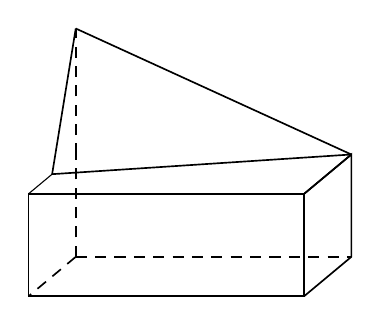
\begin{tikzpicture}[x=1cm,y=1cm,font=\normalsize,
  solid edge/.style={solid,line width=.6pt},
  hidden edge/.style={dashed,line width=.6pt,dash pattern=on 4pt off 3pt}]
\coordinate (F1) at (0,0);
\coordinate (F2) at (3.5,0);
\coordinate (F3) at (3.5,1.3);
\coordinate (F4) at (0,1.3);
\coordinate (H0) at (0.6,0.5);
\coordinate (B2) at (4.1,0.5);
\coordinate (B3) at (4.1,1.8);
\coordinate (B4) at (0.6,1.8);
\coordinate (APEX) at (0.6,3.4);
\coordinate (WL) at (0.3,1.55);
% bottom front face
\draw[solid edge] (F1) -- (F2) -- (F3) -- (F4) -- cycle;
% right face
\draw[solid edge] (F2) -- (B2) -- (B3) -- (F3);
% top face front/back edges
\draw[solid edge] (F4) -- (F3);
\draw[solid edge] (F3) -- (B3);
\draw[solid edge] (WL) -- (B3);
\draw (F4)--(WL);
% wedge left slant + apex slant
\draw[solid edge] (WL) -- (APEX);
\draw[solid edge] (APEX) -- (B3);
% hidden: back bottom, diagonal, interior vertical stubs
\draw[hidden edge] (H0) -- (F1);
\draw[hidden edge] (H0) -- (B2);
\draw[hidden edge] (H0) -- (0.6,1.8);

\draw[hidden edge] (B4) -- (APEX);
\end{tikzpicture}
